\documentclass[12pt, a4paper]{ctexrep}

% ─── 注意：本文件需使用 XeLaTeX 编译（Overleaf 中切换编译器为 XeLaTeX）────────

% ─── Packages ────────────────────────────────────────────────────────────────
\usepackage[top=2.5cm, bottom=2.5cm, left=3cm, right=2.5cm]{geometry}
\usepackage{setspace}
\usepackage{titlesec}
\usepackage{graphicx}
\graphicspath{{images/}}
\usepackage{caption}
\usepackage{subcaption}
\usepackage{float}
\usepackage{amsmath}
\usepackage{amssymb}
\usepackage{booktabs}
\usepackage{array}
\usepackage{multirow}
\usepackage{listings}
\usepackage{xcolor}
\usepackage{fancyhdr}
\usepackage{tocloft}
\usepackage{hyperref}
\usepackage{appendix}
\usepackage{cite}
\usepackage{tikz}
\usepackage{pgfplots}
\pgfplotsset{compat=1.18}

% ─── Hyperref setup ──────────────────────────────────────────────────────────
\hypersetup{
    colorlinks=true,
    linkcolor=black,
    citecolor=black,
    urlcolor=blue,
    pdftitle={直流电机串级PI控制系统},
    pdfauthor={作者姓名},
}

% ─── Page style ──────────────────────────────────────────────────────────────
\pagestyle{fancy}
\fancyhf{}
\fancyhead[L]{\small\leftmark}
\fancyhead[R]{\small\thepage}
\fancyfoot{}
\renewcommand{\headrulewidth}{0.4pt}

% ─── Line spacing ────────────────────────────────────────────────────────────
\onehalfspacing

% ─── Chapter / section title format ─────────────────────────────────────────
\titleformat{\chapter}[display]
  {\normalfont\Large\bfseries}{\chaptertitlename\ \thechapter}{12pt}{\Large}
\titlespacing*{\chapter}{0pt}{-10pt}{20pt}

% ─── Code listing style ──────────────────────────────────────────────────────
\lstdefinestyle{cstyle}{
    language=C,
    basicstyle=\ttfamily\small,
    keywordstyle=\color{blue}\bfseries,
    commentstyle=\color{gray}\itshape,
    stringstyle=\color{orange},
    numbers=left,
    numberstyle=\tiny\color{gray},
    numbersep=8pt,
    frame=single,
    breaklines=true,
    tabsize=4,
    showstringspaces=false,
    captionpos=b,
}

\lstdefinestyle{vhdlstyle}{
    language=VHDL,
    basicstyle=\ttfamily\small,
    keywordstyle=\color{blue}\bfseries,
    commentstyle=\color{gray}\itshape,
    numbers=left,
    numberstyle=\tiny\color{gray},
    numbersep=8pt,
    frame=single,
    breaklines=true,
    tabsize=4,
    captionpos=b,
}

% ─── TOC depth ───────────────────────────────────────────────────────────────
\setcounter{tocdepth}{3}
\setcounter{secnumdepth}{3}

% ─────────────────────────────────────────────────────────────────────────────
\begin{document}

% ════════════════════════════════════════════════════════════════════════════
%  封面
% ════════════════════════════════════════════════════════════════════════════
\begin{titlepage}
    \centering
    \vspace*{2cm}

    {\Large \textbf{[大学名称]}}\\[0.5cm]
    {\large [院系名称]}\\[2cm]

    \rule{\linewidth}{0.5pt}\\[0.5cm]
    {\LARGE \textbf{直流电机串级PI控制系统}}\\[0.3cm]
    {\large 基于 STM32F407 与 AX309 FPGA}\\[0.5cm]
    \rule{\linewidth}{0.5pt}\\[2cm]

    {\large
    \begin{tabular}{ll}
        \textbf{姓名：}     & [姓名] \\[0.3cm]
        \textbf{学号：}     & [学号] \\[0.3cm]
        \textbf{指导教师：} & [导师姓名] \\[0.3cm]
        \textbf{课程：}     & [课程名称] \\[0.3cm]
        \textbf{日期：}     & \today \\
    \end{tabular}
    }

    \vfill
    {\small 2025--2026 学年}
\end{titlepage}

% ════════════════════════════════════════════════════════════════════════════
%  摘要
% ════════════════════════════════════════════════════════════════════════════
\chapter*{摘要}
\addcontentsline{toc}{chapter}{摘要}
\markboth{摘要}{摘要}

本报告介绍了一种基于 STM32F407 微控制器与 AX309 FPGA 开发板的直流电机串级闭环控制系统的设计与实现。系统采用速度外环与电流内环构成的串级 PI 控制结构，实现了 0 至 100 RPM 范围内的平滑调速。

系统主要外设的初始化与数据收发采用寄存器级 C 语言实现，包括 UART、ADC、SPI、I2C 及 TIM3 正交编码器接口。FPGA 采用 VHDL 实现 12 位 PWM 发生器，PWM 频率约为 12.2\,kHz，通过 SPI 接收 STM32 发送的占空比指令。电机电流由 INA240A2 双向电流分流监视器采样后送入电流内环，编码器转速反馈则闭合速度外环。

实验结果表明：系统可在 0--100\,RPM 范围内稳定闭环运行，PWM 频率实测为 12.207\,kHz（与理论值 50\,MHz/4096 完全吻合）；在输出轴未连接外部负载、目标转速为 100\,RPM 时，系统测得电机电流约为 30\,mA。

\vspace{1em}
\noindent\textbf{关键词：}串级PI，STM32F407，FPGA，直流电机控制，电流采样，寄存器级编程，VHDL

% ════════════════════════════════════════════════════════════════════════════
%  致谢
% ════════════════════════════════════════════════════════════════════════════
\chapter*{致谢}
\addcontentsline{toc}{chapter}{致谢}
\markboth{致谢}{致谢}

% TODO: 写致谢
[在此填写致谢内容。]

% ════════════════════════════════════════════════════════════════════════════
%  目录 / 表格目录 / 图目录
% ════════════════════════════════════════════════════════════════════════════
\tableofcontents
\listoftables
\listoffigures

% ════════════════════════════════════════════════════════════════════════════
%  第一章 — 系统分析与设计
% ════════════════════════════════════════════════════════════════════════════
\chapter{系统分析与设计}

\section{功能需求与可行性分析}

本项目要实现的是一套低速直流电机闭环调速系统。用户通过旋钮电位器给定转速，STM32F407 读取电位器电压后将其换算为 0--100\,RPM 的目标转速；编码器提供实际转速反馈，电流采样放大器（INA240A2）提供电机电流反馈。控制器根据这些反馈计算 PWM 占空比，并通过 SPI 发送给 FPGA，由 FPGA 输出 PWM 信号驱动后级电机驱动模块。

围绕这一控制链路，系统需要完成以下功能：

\begin{itemize}
    \item \textbf{转速设定与闭环调速：}支持 0--100\,RPM 的目标转速设定，并根据编码器反馈自动调整 PWM 占空比，使电机转速跟随给定值。
    \item \textbf{控制精度目标：}在 PID 参数确定且负载条件稳定时，目标是减小实际转速与目标转速之间的稳态误差，具体误差通过后续实验数据进行评估。
    \item \textbf{运行状态显示：}OLED 实时显示目标转速、实际转速、PWM 占空比和电机电流，便于现场观察系统状态。
    \item \textbf{调试信息输出：}通过 UART 连接 PC，输出转速、电流、占空比及 PID 中间量，便于观察运行状态和调整 PID 参数。
    \item \textbf{参数非易失性存储：}使用 SPI Flash（W25Q64）保存 PID 参数；系统上电时会检查 Flash 中是否存在有效参数，若存在则自动读取并使用。
\end{itemize}

从硬件条件看，STM32F407 已提供本项目所需的主要接口：ADC 可用于电位器和电流信号采样，定时器可用于编码器测速和周期控制，USART、SPI 和 I2C 分别用于串口调试、外部 Flash、FPGA 通信和 OLED 显示。具体使用哪个外设实例以及对应引脚，将在后续外设映射章节中列出。执行部分由 FPGA 产生 12 位 PWM 信号，H 桥电机驱动模块（TB6612FNG）将 PWM 信号转换为电机所需的驱动电压和电流；INA240A2 电流采样模块串联在 H 桥输出与电机之间，模块上的 R100（0.1\,$\Omega$）采样电阻产生压降，经放大后送入 ADC。

从软件实现看，程序可以拆分为采样、滤波、控制、通信、显示和参数存储等模块。周期控制任务负责读取输入与反馈信号，并根据串级 PI 的计算结果输出 PWM 控制量；串口命令处理、OLED 刷新和 Flash 参数保存则放在主循环中完成。这样可以让闭环控制和显示、存储等任务分开实现，程序结构也更清楚。

综上，本项目在硬件接口和软件任务划分上具备实现条件。稳态误差、电流测量和参数保存等结果将在实验章节中进一步验证。

\section{系统架构设计}

系统采用分层架构，如图~\ref{fig:arch} 所示。

\begin{figure}[H]
    \centering
    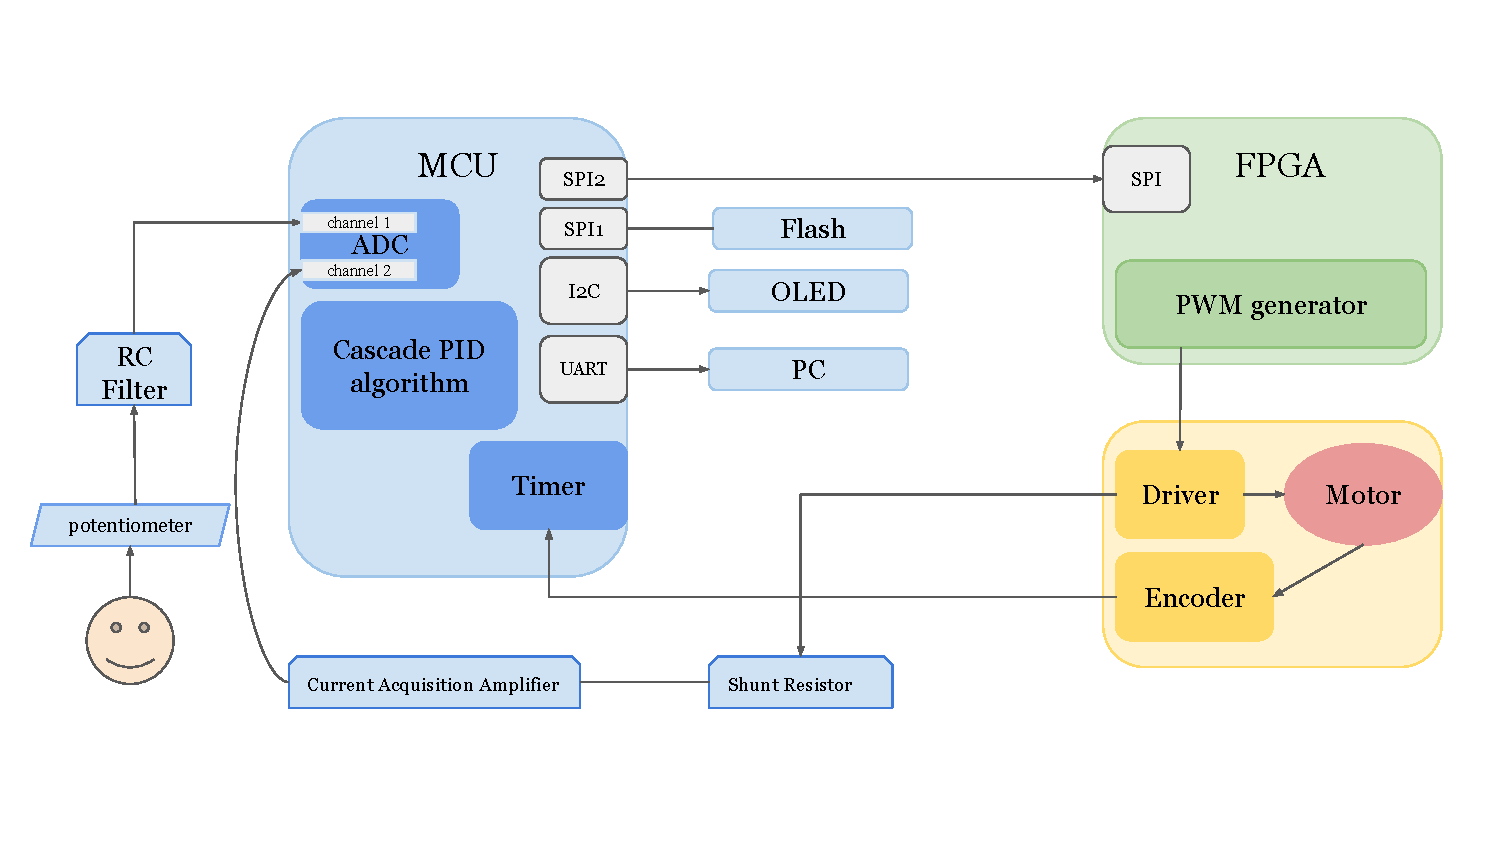
\includegraphics[width=0.95\textwidth]{architecture.pdf}
    \caption{直流电机串级 PI 控制系统架构图。}
    \label{fig:arch}
\end{figure}

系统主要由 MCU 控制部分、FPGA PWM 发生部分和电机执行部分组成。电位器输出先经过 RC 滤波，再接入 MCU 的 ADC 通道 1，用作目标转速输入；INA240A2 模块串联在 H 桥输出与电机之间，模块输出接入 ADC 通道 2，用作电流反馈；编码器 A/B 相接入 MCU 的定时器编码器接口，用于计算实际转速。MCU 根据目标转速、实际转速和电流反馈完成串级 PI 运算，并通过 SPI2 将占空比指令发送给 FPGA。FPGA 生成 PWM 信号后驱动 H 桥电机驱动模块，最终控制直流电机运行。W25Q64 Flash、OLED 和 PC 分别通过 SPI1、I2C 和 UART 与 MCU 连接，用于 PID 参数存储、状态显示和串口调试。

主控制链路如下：
\[
\text{电位器} \xrightarrow{\text{RC + ADC}} \text{STM32 PID}
\xrightarrow{\text{SPI2}} \text{FPGA} \xrightarrow{\text{PWM}}
\text{TB6612} \rightarrow \text{电机}
\]
编码器转速与电流采样信号则反馈至 STM32，形成闭环控制。

\section{控制策略：串级PI}

若只采用单环速度 PI，控制链路可以表示为：

\[
\text{目标转速}
\rightarrow \text{速度 PI}
\rightarrow \text{PWM}
\rightarrow \text{电机}
\]

这种结构能够调节转速，但它只根据编码器反馈修正 PWM。编码器反映的是机械运动结果，受转子惯量和负载影响，变化相对较慢；电机电流则是电气量，PWM 增大后会更快上升。因此在启动或负载突变时，转速反馈可能还没有明显变化，电流已经先升高，单环速度 PI 难以及时约束电流。

为此，本项目在速度环和 PWM 之间加入电流环，形成串级 PI：

\[
\text{目标转速}
\rightarrow \text{速度 PI}
\rightarrow \text{目标电流}
\rightarrow \text{电流 PI}
\rightarrow \text{PWM}
\rightarrow \text{电机}
\]

其中，编码器转速反馈给速度 PI，电流采样结果反馈给电流 PI。速度外环根据转速误差给出目标电流，表示当前为了接近目标转速需要多大的驱动力；电流内环再根据目标电流和实际电流计算 PWM，占空比不再直接由转速误差决定。

这两个闭环的分工是：速度外环负责转速目标，电流内环负责实际电流。由于电流变化快于转速变化，电流环能够更早感知启动或负载变化带来的电流上升，并根据实际电流调节 PWM；同时目标电流本身设有上限，因此可以减少电流过大对电机和驱动电路造成的压力。

% ════════════════════════════════════════════════════════════════════════════
%  第二章 — 硬件架构与模块实现
% ════════════════════════════════════════════════════════════════════════════
\chapter{硬件架构与模块实现}

本章在系统架构图的基础上，进一步说明各硬件模块的具体实现和连接关系。内容依次包括输入与反馈链路、MCU 外设与引脚分配、FPGA PWM 发生模块、电机驱动电路以及电源连接方式。寄存器级外设驱动将在下一章展开，控制算法的具体公式与限幅处理则在后续控制算法章节说明。

\section{输入与反馈传感链路}

\subsection{电位器与 RC 低通滤波器}

旋钮电位器连接至 PA0（ADC1\_IN0），作为目标转速给定输入。由于电位器滑动端在机械转动时可能存在接触抖动，面包板供电中也含有数字电路开关噪声，若直接接入 ADC 容易造成采样值跳动。因此，电位器输出先经过 RC 低通滤波器（$f_c = 1/(2\pi RC)$），在进入 ADC 前衰减高频干扰。

\IfFileExists{images/breadboard_connection.pdf}{
    \begin{figure}[H]
        \centering
        \includegraphics[width=0.85\textwidth]{images/breadboard_connection.pdf}
        \caption{输入与反馈传感链路的实物连接图。}
        \label{fig:breadboard_connection}
    \end{figure}
}{}

\begin{figure}[H]
    \centering
    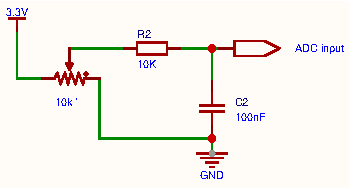
\includegraphics[width=0.85\textwidth]{images/adc_Rc.pdf}
    \caption{电位器转速给定输入及 RC 低通滤波电路。}
    \label{fig:sensor_schematic}
\end{figure}

\subsection{电流传感：INA240A2 电流采样模块}

本项目使用带 R100 采样电阻的 INA240A2 电流采样模块。模块中的 R100 与电机串联，连接关系为
\[
\text{AO1} \rightarrow \text{R100} \rightarrow \text{电机} \rightarrow \text{AO2}.
\]
因此，电机电流会全部流过 R100。INA240A2 的 IN+ 和 IN- 分别连接在 R100 两端，用于测量该电阻上的压差；其输入端只负责测量，电机的主要电流不会流入 INA240A2 芯片。这种接法直接测量 H 桥输出回路中的电机电流，不属于普通的电源高边或接地低边采样。

R100 的阻值为 0.1\,$\Omega$，电流流过时会产生与电流成正比的微小压降。以 30--300\,mA 的工作电流估算，该压降约为 3--30\,mV。INA240A2 将 IN+ 与 IN- 之间的差分电压放大 50 倍，再通过 OUT 引脚送入 STM32 的 PA1（ADC1\_IN1），使电流变化能够被稳定测量。

\begin{figure}[H]
    \centering
    \includegraphics[width=0.85\textwidth]{images/current_amplifier.pdf}
    \caption{H 桥输出侧的 INA240A2 电流采样链路。}
    \label{fig:ina240}
\end{figure}

INA240A2 的输出电压可表示为：

\begin{equation}
    V_{\text{out}} = V_{\text{ref}} + G \cdot I \cdot R_{\text{shunt}}
    \label{eq:ina240_out}
\end{equation}

模块内部已将 REF1 接 GND、REF2 接 VCC，因此理论零电流基准为 $V_{\text{ref}} = V_{\text{CC}}/2$。在电机无电流时，STM32 通过 PA1（ADC1\_IN1）读取到的原始值约为 2200；按 3.3\,V ADC 满量程换算，INA240A2 的零电流输出约为 $1773\,\text{mV}$。软件使用该值进行零点校准，电机电流计算公式为：

\begin{equation}
    I\,[\text{mA}] = \frac{V_{\text{out}}\,[\text{mV}] - 1773}
                         {50 \times 0.1}
                  = \frac{V_{\text{out}} - 1773}{5}
    \label{eq:current}
\end{equation}

在电机输出轴未连接外部负载、目标转速为 100\,RPM 时，系统测得电机电流约为 30\,mA。电机手册给出的 12\,V 空载电流约为 70\,mA，但该数据对应约 280\,RPM 的全速空载工况。由于本项目通过 PWM 将转速限制在 100\,RPM，两者测试条件不同，因此手册数据仅作为量级参考。

\subsection{转速传感：编码器与 TIM3 正交解码}

JGA25-370 电机内置霍尔效应正交编码器，输出 A、B 两相信号。编码器安装在电机内部轴上，而控制对象是减速后的输出轴，因此转速计算需要同时考虑编码器每转脉冲数和齿轮减速比。本项目电机编码器为 11\,PPR，减速比为 34，TIM3 编码器模式对 A/B 相四个边沿计数，因此输出轴每转对应
\[
    11 \times 34 \times 4 = 1496
\]
个计数。

若采用 GPIO 外部中断处理，每个边沿都会触发 CPU 中断，电机转速升高时会明显占用控制循环时间。TIM3 配置为编码器模式 3（SMS = 011），由硬件状态机完成 A/B 相解码。CPU 只需在控制中断中读取一次 CNT 差值即可计算转速，开销很小；同时硬件数字滤波器（IC1F = IC2F = 0001，2 采样）用于抑制短脉冲干扰。转速计算公式为：

\begin{equation}
    \text{RPM} = \frac{\Delta_{\text{count}} \times 60{,}000}
                      {N_{\text{PPR}}}
    \label{eq:rpm}
\end{equation}

其中 $\Delta_{\text{count}}$ 为有符号 16 位计数器差值（自动处理溢出），$N_{\text{PPR}}$ 为每转脉冲数（含减速比与 $\times4$ 模式）。

\section{MCU 控制核心（STM32F407G-DISC1）}

\subsection{MCU 选型与规格}

STM32F407VG（Cortex-M4，168\,MHz，带 FPU）外设资源丰富，处理能力足以完成本项目的 1\,kHz 控制任务。本项目使用的主要外设如表~\ref{tab:mcu_periph} 所示。

\begin{table}[H]
    \centering
    \caption{本项目使用的 STM32F407 外设。}
    \label{tab:mcu_periph}
    \begin{tabular}{lll}
        \toprule
        \textbf{外设} & \textbf{功能} & \textbf{工作频率/通信速率} \\
        \midrule
        TIM6   & 1\,kHz PI 控制中断 & TIM6CLK = 84\,MHz，输出 1\,kHz \\
        TIM3   & 正交编码器接口       & TIM3CLK = 84\,MHz，外部 A/B 相计数 \\
        ADC1   & 电位器 + 电流采样    & ADC clock = 21\,MHz \\
        SPI1   & W25Q64 Flash& SCK = 5.25\,MHz \\
        SPI2   & FPGA 占空比传输      & SCK = 5.25\,MHz \\
        I2C1   & OLED SSD1306 显示屏  & 目标 SCL = 100\,kHz \\
        USART2 & 串口调试（CH340G）   & 115200 baud \\
        \bottomrule
    \end{tabular}
\end{table}

\subsection{引脚分配与外设映射}

表~\ref{tab:pins} 列出了全部 16 个信号引脚的分配情况。

\begin{table}[H]
    \centering
    \caption{STM32F407 引脚分配表。}
    \label{tab:pins}
    \begin{tabular}{lll}
        \toprule
        \textbf{引脚} & \textbf{外设} & \textbf{连接对象} \\
        \midrule
        PA0  & ADC1\_IN0   & 电位器（经 RC 滤波后接入） \\
        PA1  & ADC1\_IN1   & INA240A2 输出 \\
        PA2  & USART2\_TX  & CH340G RXD \\
        PA3  & USART2\_RX  & CH340G TXD \\
        PA4  & SPI1\_CS    & W25Q64 片选（软件 NSS） \\
        PA5  & SPI1\_SCK   & W25Q64 时钟 \\
        PA6  & SPI1\_MISO  & W25Q64 数据输出 \\
        PA7  & SPI1\_MOSI  & W25Q64 数据输入 \\
        PB6  & I2C1\_SCL   & OLED SCL \\
        PB7  & I2C1\_SDA   & OLED SDA \\
        PB12 & SPI2\_CS    & FPGA cs\_n（软件 NSS） \\
        PB13 & SPI2\_SCK   & FPGA sck \\
        PB14 & SPI2\_MISO  & FPGA miso（不使用） \\
        PB15 & SPI2\_MOSI  & FPGA mosi \\
        PC6  & TIM3\_CH1   & 编码器 A 相 \\
        PC7  & TIM3\_CH2   & 编码器 B 相 \\
        \bottomrule
    \end{tabular}
\end{table}

\section{FPGA PWM 发生模块（AX309 Spartan-6）}

\subsection{FPGA 的角色}

STM32F407 自带硬件 PWM 定时器，单纯从功能上也可以直接输出 PWM。本项目将 PWM 发生部分放在 FPGA 中实现，主要是为了验证 SPI 从机接收逻辑和 12 位 PWM 比较器。FPGA 接收 STM32 通过 SPI2 发送的占空比数值，并在完整数据帧结束后更新 PWM 输出。

AX309 开发板通过 J3 扩展口与 STM32 和电机驱动模块连接，关键引脚如表~\ref{tab:fpga_pins} 所示。

\begin{table}[H]
    \centering
    \caption{AX309 FPGA 关键引脚连接。}
    \label{tab:fpga_pins}
    \begin{tabular}{llll}
        \toprule
        \textbf{信号} & \textbf{FPGA 引脚} & \textbf{J3 针脚} & \textbf{连接对象} \\
        \midrule
        sck      & C15 & J3-21 & STM32 PB13（SPI2\_SCK） \\
        cs\_n    & D16 & J3-23 & STM32 PB12（SPI2\_CS） \\
        mosi     & C16 & J3-24 & STM32 PB15（SPI2\_MOSI） \\
        miso     & E15 & J3-26 & STM32 PB14（SPI2\_MISO，未使用） \\
        pwm\_out & F16 & J3-31 & TB6612FNG PWMA \\
        \bottomrule
    \end{tabular}
\end{table}

\subsection{PWM 频率}

AX309 开发板板载 50\,MHz 晶振。12 位计数器计至 4096 后归零，因此：

\begin{equation}
    f_{\text{PWM}} = \frac{f_{\text{clk}}}{2^{12}} = \frac{50 \times 10^6}{4096}
    \approx 12.207\,\text{kHz}
    \label{eq:pwm_freq}
\end{equation}

该频率高于常见低频电机嗡声范围，但仍处于部分人耳可感知的频段；其优势主要在于开关周期短、12 位分辨率足够细（最低有效位 $= 100\,\%/4096 \approx 0.024\,\%$），可实现较平滑的调速。逻辑分析仪实测值：12.207\,kHz，与理论值完全吻合。

\section{电机驱动电路（TB6612FNG）}

FPGA 输出的 PWM 仅是 3.3\,V 逻辑控制信号，无法直接为电机供电。JGA25-370 电机使用 12\,V 电源，运行电流也明显高于 FPGA 引脚能够提供的电流，因此系统在 FPGA 与电机之间加入 TB6612FNG 电机驱动器。FPGA 负责给出 PWM 控制信号，TB6612FNG 则根据该信号控制 12\,V 电机电源，并向电机提供实际所需的驱动电流。

PWM 信号接入 TB6612FNG 的 PWMA 引脚。当 PWM 为高电平时，驱动器向电机施加电压；当 PWM 为低电平时，驱动器进入相应的关断或续流状态。由于这一过程快速重复，电机线圈中的电流不会随每次开关立即突变，电机获得的等效平均电压可近似表示为

\begin{equation}
    U_{\text{avg}} \approx D \times 12\,\text{V},
\end{equation}

其中 $D$ 为 PWM 占空比。典型占空比对应的等效平均电压如表~\ref{tab:pwm_voltage} 所示。

\begin{table}[H]
    \centering
    \caption{PWM 占空比与等效平均电压的关系。}
    \label{tab:pwm_voltage}
    \begin{tabular}{ccc}
        \toprule
        \textbf{占空比} & \textbf{等效平均电压} & \textbf{电机状态} \\
        \midrule
        0\%   & 0\,V  & 停止驱动 \\
        25\%  & 约 3\,V  & 低速运行 \\
        50\%  & 约 6\,V  & 中等占空比运行 \\
        100\% & 约 12\,V & 全占空比运行 \\
        \bottomrule
    \end{tabular}
\end{table}

占空比增大时，电机获得的平均电压随之提高，通常表现为转速和输出转矩增加。因此，本系统通过改变 PWM 占空比实现电机调速。

TB6612FNG 的 H 桥结构本身支持电机正反转，但本项目只使用单向调速，其控制引脚配置见表~\ref{tab:tb6612}。FPGA 不控制电机方向，只通过 PWMA 引脚调节占空比。图~\ref{fig:h_bridge} 中的 VDD 和 Load 分别对应本项目的 12\,V 电机电源和直流电机，AO1、AO2 为连接电机回路的两个 H 桥输出端。

\begin{figure}[H]
    \centering
    \includegraphics[width=0.55\textwidth]{images/H_principle.png}
    \caption{H 桥电机驱动基本原理。}
    \label{fig:h_bridge}
\end{figure}

\begin{table}[H]
    \centering
    \caption{TB6612FNG 控制信号接线表。}
    \label{tab:tb6612}
    \begin{tabular}{lll}
        \toprule
        \textbf{TB6612 引脚} & \textbf{连接对象} & \textbf{说明} \\
        \midrule
        PWMA    & FPGA J3-31（F16） & FPGA 输出 PWM 占空比 \\
        AIN1    & 3.3\,V            & 方向：正转 \\
        AIN2    & GND               & 方向：正转 \\
        STBY    & 3.3\,V            & 必须拉高，否则芯片待机不工作 \\
        VCC     & 3.3\,V            & 驱动器逻辑电源 \\
        VM      & 12\,V 电源        & 电机驱动电源 \\
        GND     & 公共地            & 与 STM32、FPGA 和电流采样模块共地 \\
        AO1     & INA240A2 模块 IN+ & 经采样模块连接电机 \\
        AO2     & 电机另一端         & 构成完整 H 桥输出回路 \\
        \bottomrule
    \end{tabular}
\end{table}

\section{电源设计与噪声抑制}

系统采用功率电源与逻辑电源分开供电、各模块共地的方式。STM32F407G-DISC1 和 AX309 FPGA 开发板分别通过 USB 连接 PC 供电；TB6612FNG 的 VM 引脚由外部可调直流稳压电源提供 12\,V 电压，用于驱动电机，其 VCC 引脚接 3.3\,V 逻辑电源。

电机启动和 PWM 调速会产生电流突变及电源波动。将电机功率电源与 MCU、FPGA 的逻辑电源分开，可以减小这些干扰对数字通信和 ADC 采样的影响。各模块仍需保持公共地，使 PWM、SPI 和 ADC 等信号具有统一的电平参考。

% ════════════════════════════════════════════════════════════════════════════
%  第三章 — 嵌入式软件开发
% ════════════════════════════════════════════════════════════════════════════
\chapter{MCU 寄存器级软件开发}

本章说明 MCU 侧各外设的实现。USART、ADC、SPI、I2C 和定时器的初始化及数据收发主要通过寄存器完成，延时等基础功能沿用工程已有的系统函数。

\section{寄存器级外设驱动}

\subsection{UART}

串口用于向 PC 输出目标转速、实际转速、电流、占空比及 PID 中间量，便于观察系统运行状态。根据 RM0090 中 USART 外设的配置要求，并结合 DS8626 的引脚复用表，本项目选用 USART2，配置结果如表~\ref{tab:usart2_config} 所示。

\begin{table}[H]
    \centering
    \caption{USART2 功能需求与配置。}
    \label{tab:usart2_config}
    \begin{tabular}{lll}
        \toprule
        \textbf{功能需求} & \textbf{配置} & \textbf{对应设置} \\
        \midrule
        串口发送与接收 & PA2（TX）、PA3（RX） & GPIOA AF7 \\
        外设时钟       & GPIOA、USART2       & AHB1、APB1 时钟使能 \\
        通信速率       & 115200\,baud        & 配置 \texttt{BRR} \\
        数据格式       & 8N1                 & 8 位、无校验、1 位停止位 \\
        收发使能       & 发送、接收同时启用   & \texttt{TE}、\texttt{RE}、\texttt{UE} 置 1 \\
        \bottomrule
    \end{tabular}
\end{table}

PA2 和 PA3 配置为 AF7、推挽输出且无上下拉。根据 RM0090，\texttt{USART\_CR1} 中 \texttt{OVER8} 位的复位值为 0，对应 16 倍过采样。本项目未修改该位，因此 APB1 时钟为 42\,MHz 时，波特率寄存器计算如下：
\begin{equation}
    \text{USARTDIV} = \frac{f_{\text{APB1}}}{16 \times \text{BaudRate}}
    = \frac{42{,}000{,}000}{16 \times 115{,}200} \approx 22.786
    \quad\Rightarrow\quad \texttt{BRR = 0x16D}
\end{equation}

发送函数等待 \texttt{SR} 寄存器的 \texttt{TXE} 标志位置 1 后，再向 \texttt{DR} 寄存器写入数据，避免覆盖尚未发送的字节。USART2 通过外接 CH340G USB 转串口模块与 PC 连接，其中 PA2 接 CH340G 的 RXD，PA3 接 TXD，并保持共地。串口参数为 115200\,baud、8N1。

\subsection{ADC}

STM32F407 内部包含 ADC1、ADC2 和 ADC3 三个 ADC 外设实例，每个实例都有独立的控制与数据寄存器。本项目只使用 ADC1，并选择其中两个输入通道：PA0 对应 ADC1\_IN0，用于采集电位器电压；PA1 对应 ADC1\_IN1，用于采集电流反馈。

程序先通过 ADC1 的 \texttt{SQR3} 寄存器选择输入通道，再将 \texttt{SWSTART} 位置 1，启动一次转换。转换完成后，程序等待 \texttt{EOC} 标志置 1，并从 \texttt{DR} 寄存器读取 0--4095 的 12 位结果。

STM32F407 的片内 ADC 采用逐次逼近型（SAR）结构。采样阶段，内部采样电容连接输入并保存当前电压；转换阶段，SAR 逻辑从最高位开始给出试探数字，内部 DAC 将其转换为试探电压，比较器再将该电压与采样电压比较。SAR 根据比较结果保留或清除当前位，并继续判断下一位。经过 12 次比较后，得到最终的 12 位数字结果。其基本结构如图~\ref{fig:sar_adc} 所示。

\begin{figure}[H]
    \centering
    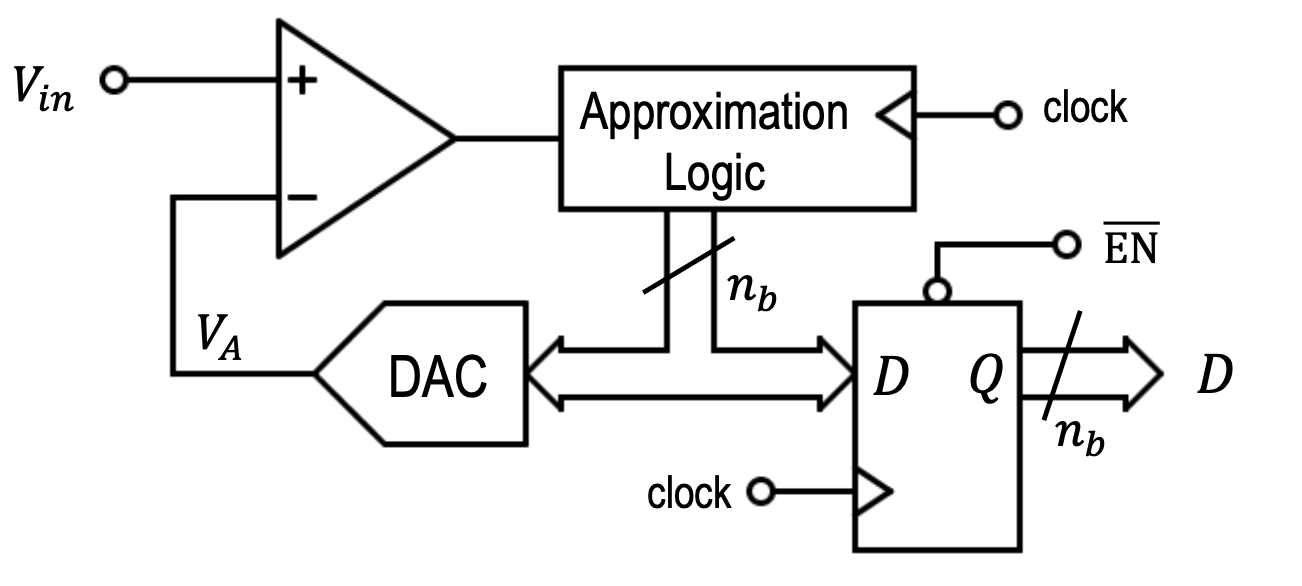
\includegraphics[width=0.85\textwidth]{images/sar.png}
    \caption{SAR ADC 的基本结构。}
    \label{fig:sar_adc}
\end{figure}

ADC 时钟由 APB2 时钟经过公共预分频器产生。APB2 时钟为 84\,MHz，而数据手册规定 ADC 时钟最高为 36\,MHz，因此不能采用 2 分频得到 42\,MHz。本项目将 \texttt{ADC\_CCR} 的 \texttt{ADCPRE} 配置为 4 分频，使 ADC 时钟为
\[
    f_{\text{ADCCLK}}=\frac{84\,\text{MHz}}{4}=21\,\text{MHz},
\]
对应的单个 ADC 时钟周期约为 $1/21\,\text{MHz}=47.6\,\text{ns}$。

采样时间表示 ADC 内部采样电容与输入信号连接的时间，其单位为 ADC 时钟周期。输入源阻抗越高，通常需要更长时间使采样电容充分充电。电位器输出经过由 10\,k$\Omega$ 电阻和 100\,nF 电容组成的 RC 低通滤波器后接入 ADC，因此采用较长的 144 周期；电流采样放大器输出阻抗较低，采用 28 周期。两个通道的配置见表~\ref{tab:adc_config}。

\begin{table}[H]
    \centering
    \caption{ADC1 双通道采样配置。}
    \label{tab:adc_config}
    \begin{tabular}{llll}
        \toprule
        \textbf{采样对象} & \textbf{引脚与通道} & \textbf{采样时间} & \textbf{用途} \\
        \midrule
        电位器输出       & PA0 / ADC1\_IN0 & 144 周期（约 6.86\,$\mu$s） & 计算目标转速 \\
        电流采样放大器输出 & PA1 / ADC1\_IN1 & 28 周期（约 1.33\,$\mu$s） & 计算电机电流 \\
        \bottomrule
    \end{tabular}
\end{table}

12 位转换过程还需要 12 个 ADC 时钟周期，因此两个通道的单次总转换时间分别约为 7.43\,$\mu$s 和 1.90\,$\mu$s。本项目通过 TIM6 每 1\,ms 产生一次中断，在中断中依次读取电位器、转速和电流反馈，完成 PID 计算并更新 PWM 指令。两路 ADC 转换合计约 9.33\,$\mu$s，占这 1\,ms 的比例不足 1\%，不会明显影响其余计算。TIM6 的具体配置将在后文定时器小节中说明。

\subsection{SPI}

STM32 分别通过 SPI1 与 W25Q64 Flash 通信，通过 SPI2 向 FPGA 发送 12 位占空比。两路 SPI 的主要配置和用途见表~\ref{tab:spi_compare}。

\begin{table}[H]
    \centering
    \caption{SPI1 与 SPI2 配置对比。}
    \label{tab:spi_compare}
    \begin{tabular}{lllll}
        \toprule
        \textbf{接口} & \textbf{通信对象} & \textbf{时钟频率} & \textbf{片选} & \textbf{数据方向} \\
        \midrule
        SPI1 & W25Q64 Flash & 5.25\,MHz & PA4  & 双向 \\
        SPI2 & FPGA         & 5.25\,MHz & PB12 & 单向发送 \\
        \bottomrule
    \end{tabular}
\end{table}

SPI1 挂载在 APB2 总线上，时钟为 84\,MHz。\texttt{SPI1\_CR1} 中的 \texttt{BR[2:0]} 配置为 \texttt{011}，对应 16 分频，因此
\[
    f_{\text{SPI1}}=\frac{84\,\text{MHz}}{16}=5.25\,\text{MHz}.
\]
SPI2 挂载在 APB1 总线上，时钟为 42\,MHz。\texttt{SPI2\_CR1} 中的 \texttt{BR[2:0]} 配置为 \texttt{010}，对应 8 分频，因此
\[
    f_{\text{SPI2}}=\frac{42\,\text{MHz}}{8}=5.25\,\text{MHz}.
\]

两路接口均由 STM32 作为主机，配置为 Mode 0、8 位数据帧和 MSB 优先，并使用 GPIO 软件控制片选。

\subsubsection{SPI1}

PID 参数在程序运行时保存在 SRAM 中，但 SRAM 断电后数据会丢失，重新上电后无法保留已经调好的参数。STM32 内部 Flash 主要用于存放程序，本项目因此使用独立的 W25Q64 保存 PID 参数，使参数存储与程序存储分开。W25Q64 断电后仍能保留数据，并可通过 SPI1 读写；用户保存参数后，系统能够在下次上电时读取并继续使用。

SPI 是一种同步全双工串行协议：主机（STM32）负责产生时钟 SCK 和片选 CS，数据在 SCK 上升沿按 MSB 优先移位（Mode 0）；MOSI 承载主机到从机的数据，MISO 承载从机到主机的数据，CS 拉低表示选中该从机、CS 拉高表示事务结束。W25Q64 作为 SPI 从机不会主动发起通信，所有操作均由 STM32 以 CS↓ + 指令字节 + 地址 + 数据 + CS↑ 的完整帧格式主动发起。

通信时序为：拉低片选引脚（选中从机）$\to$ 收发数据字节 $\to$ 拉高片选引脚（释放从机）。

W25Q64FV 是容量为 8\,MB 的 NOR Flash。其基本存储单元为浮栅晶体管，浮栅被绝缘层包围，能够在断电后保留电子。浮栅中的电荷会改变晶体管的阈值电压，读取电路通过判断晶体管在给定电压下是否导通来识别 0 和 1。

图~\ref{fig:nor_flash_programming}给出了 NOR Flash 阵列的编程过程。地址译码器根据输入地址选中目标字线，并对需要写为 0 的位线施加编程电压，使对应晶体管通过热电子注入完成编程。同一字线中需要变为 0 的多个存储位可以同时编程。

\begin{figure}[H]
    \centering
    \includegraphics[width=0.4\textwidth]{images/flash1.png}
    \caption{NOR Flash 阵列的字线选择与位编程原理。}
    \label{fig:nor_flash_programming}
\end{figure}

图~\ref{fig:flash_tunneling}给出了浮栅晶体管的擦除过程。擦除时，浮栅中的电子在强电场作用下通过薄氧化层发生 Fowler--Nordheim 隧穿，电子离开浮栅后，晶体管的阈值电压降低，存储位由 0 恢复为 1。

\begin{figure}[H]
    \centering
    \includegraphics[width=0.4\textwidth]{images/flash2.png}
    \caption{FLOTOX 浮栅晶体管的 F--N 隧穿擦除过程。}
    \label{fig:flash_tunneling}
\end{figure}

因此，NOR Flash 的编程操作只能将存储位由 1 改为 0；若要将 0 恢复为 1，则必须先擦除相应扇区。

本项目使用的主要指令见表~\ref{tab:w25q64_commands}。

\begin{table}[H]
    \centering
    \caption{W25Q64 主要操作指令。}
    \label{tab:w25q64_commands}
    \begin{tabular}{lll}
        \toprule
        \textbf{操作} & \textbf{指令码} & \textbf{说明} \\
        \midrule
        读 ID    & \texttt{0x90} & 返回制造商和器件标识 \\
        写使能   & \texttt{0x06} & 写入或擦除前使 WEL 位置 1 \\
        读数据   & \texttt{0x03} & 从指定地址连续读取数据 \\
        页编程   & \texttt{0x02} & 一次最多写入 256 字节 \\
        扇区擦除 & \texttt{0x20} & 将一个 4\,KB 扇区恢复为 1 \\
        \bottomrule
    \end{tabular}
\end{table}

每次写入或擦除前必须先发送写使能指令，使 WEL 位置 1。由于扇区擦除会将整个 4\,KB 区域恢复为 1，因此更新 PID 参数时先擦除目标扇区，再执行页编程。

\begin{figure}[H]
    \centering
    \includegraphics[width=0.95\textwidth]{images/flash_page.png}
    \caption{W25Q64 页编程指令时序（SPI Mode）。}
    \label{fig:flash_page_program}
\end{figure}

如图~\ref{fig:flash_page_program}所示，页编程事务依次发送 \texttt{0x02} 指令、24 位地址和 1--256 字节数据，随后将 CS 拉高以启动芯片内部的编程操作。该图描述的是一条页编程指令内部的数据帧。根据数据手册，在页编程或扇区擦除命令结束后，开始读取状态寄存器前，CS 应保持高电平至少 50\,ns，该时间记为 $t_{\mathrm{SHSL}}$。

调试过程中曾出现 Flash 读取正常但写入和擦除失败的问题。检查后发现，写入或擦除命令结束后过早读取状态寄存器，未满足上述片选间隔。程序在相关事务结束后加入 1\,ms 延时，该延时远大于 50\,ns 的最低要求；修改后，写入和断电回读恢复正常。

PID 参数存放在 Flash 扇区 0 的起始位置（地址 \texttt{0x000000}），共占用 32\,字节。其中包括一个有效标志、速度环的三个 PID 参数、电流环的三个 PID 参数以及一个保留位置。有效标志使用固定值 \texttt{12345.678f}，用于判断该区域是否保存过有效数据。系统上电后先检查该标志；标志正确时读取六个 PID 参数，否则使用程序中的默认参数。

\subsubsection{SPI2}

SPI2 使用项目自定义的两字节协议向 FPGA 发送占空比。CS 边沿作为帧定界符，FPGA 在 CS 上升沿锁存完整的 12 位占空比值，数据帧格式见表~\ref{tab:spi2_frame}。

\begin{table}[H]
    \centering
    \caption{SPI2 占空比数据帧格式。}
    \label{tab:spi2_frame}
    \begin{tabular}{lll}
        \toprule
        \textbf{传输顺序} & \textbf{位段} & \textbf{内容} \\
        \midrule
        字节 0 & [7:4] & 固定为 \texttt{0000} \\
        字节 0 & [3:0] & \texttt{duty[11:8]} \\
        字节 1 & [7:0] & \texttt{duty[7:0]} \\
        \bottomrule
    \end{tabular}
\end{table}

PWM 占空比为 12 位，而 SPI2 每次发送 8 位数据，因此 STM32 将占空比拆成两个字节发送。第一个字节的低 4 位存放占空比的高 4 位，其余 4 位补零；第二个字节存放占空比的低 8 位。FPGA 接收两个字节后，将对应位重新拼接为完整的 12 位占空比。

SPI2 配置为 APB1/8 = 5.25\,MHz，模式 0，8 位 MSB 优先。由于 FPGA 不回传数据，MISO（PB14）可不接线。

\subsection{I2C}

本项目使用 I2C1 驱动 SSD1306 OLED。STM32 是主机，负责产生时钟并发送地址和显示数据；OLED 是从机，地址匹配后返回应答并接收数据。本项目只向 OLED 写入命令和显示数据，不读取 OLED 内容。与 SPI 通过独立片选信号选择设备不同，I2C 在共享总线上发送 7 位地址来选择从机，因此 OLED 不需要单独的片选引脚。

SCL 和 SDA 均采用开漏输出。设备可以主动将总线拉低，输出高电平时则释放总线，由上拉电阻将线路拉高。这样多个设备可以共用总线而不会因输出电平相反造成短路。SCL 为高电平时，SDA 由高变低表示 START，SDA 由低变高表示 STOP；正常传输期间，SDA 只在 SCL 为低时改变。每发送 8 位数据后，发送方释放 SDA，OLED 在第 9 个时钟周期将 SDA 拉低表示 ACK。

I2C1 的主要配置见表~\ref{tab:i2c_config}。

\begin{table}[H]
    \centering
    \caption{I2C1 与 SSD1306 通信配置。}
    \label{tab:i2c_config}
    \begin{tabular}{lll}
        \toprule
        \textbf{项目} & \textbf{配置} & \textbf{说明} \\
        \midrule
        引脚       & PB6（SCL）、PB7（SDA） & AF4、开漏输出 \\
        OLED 地址  & \texttt{0x3C}           & 写地址字节为 \texttt{0x78} \\
        控制字节   & \texttt{0x00}/\texttt{0x40} & 命令/显示数据 \\
        APB1 时钟  & 42\,MHz                 & I2C1 外设时钟来源 \\
        目标 SCL   & 100\,kHz                & 标准模式 \\
        \bottomrule
    \end{tabular}
\end{table}

SSD1306 的 7 位地址为 \texttt{0x3C}。发送写操作时，程序将该地址左移一位，并在最低位写入读写标志 0，因此总线上实际发送的地址字节为
\[
    (\texttt{0x3C} \ll 1) \,|\, 0 = \texttt{0x78}.
\]
地址之后还需发送一个控制字节：\texttt{0x00} 表示后续内容是 OLED 命令，\texttt{0x40} 表示后续内容是显示数据。

\begin{figure}[H]
    \centering
    \includegraphics[width=0.92\textwidth]{images/iic.png}
    \caption{I2C 主机读写操作的总线时序。}
    \label{fig:i2c_read_write}
\end{figure}

图~\ref{fig:i2c_read_write}同时给出了主机写和主机读两种时序。主机写操作中，地址和数据由主机发送，ACK 由从机返回；主机读操作中，数据由从机发送，ACK 或 NACK 由主机产生。本项目只使用图中的主机写操作：STM32 依次发送 OLED 地址、控制字节和命令或显示数据，每发送一个字节后由 OLED 返回 ACK，最后由 STM32 产生 STOP 条件。

I2C1 位于 APB1 总线，输入时钟为 42\,MHz。根据 RM0090，I2C 标准模式支持的最高 SCL 频率为 100\,kHz，本项目按该频率配置，因此
\[
    \texttt{CCR}=\frac{42\,\text{MHz}}{2\times100\,\text{kHz}}=210.
\]
RM0090 同时规定，标准模式下 SCL 的最大上升时间为 1000\,ns。该时间对应 42 个 APB1 时钟周期，因此 \texttt{TRISE} 配置为 $42+1=43$。程序最终将 \texttt{CR2}、\texttt{CCR} 和 \texttt{TRISE} 分别配置为 42、210 和 43。

发送数据时，CPU 将地址、控制字节和数据依次写入 \texttt{I2C1->DR}。I2C1 外设按照 I2C 协议完成数据移位和时序控制，SCL 和 SDA 信号分别由 PB6 和 PB7 输出至 OLED。OLED 接收后更新内部控制器或显存。通信过程中对等待总线空闲、START、地址应答和数据发送等步骤设置超时；发生异常时产生 STOP 并清除错误标志，避免 OLED 通信故障使程序一直停在等待状态。

\subsection{定时器}

本项目使用 TIM3 完成编码器计数，使用 TIM6 周期触发控制循环，配置见表~\ref{tab:timer_config}。

\begin{table}[H]
    \centering
    \caption{定时器功能与配置。}
    \label{tab:timer_config}
    \begin{tabular}{llll}
        \toprule
        \textbf{定时器} & \textbf{功能} & \textbf{主要配置} & \textbf{结果} \\
        \midrule
        TIM3 & 编码器脉冲计数 & PC6/PC7，编码器模式 3 & 四倍频计数 \\
        TIM6 & 周期控制中断   & PSC=83，ARR=999       & 1\,kHz 更新中断 \\
        \bottomrule
    \end{tabular}
\end{table}

TIM3 对编码器 A、B 两相信号的上升沿和下降沿进行计数，并启用输入数字滤波以抑制短时干扰。TIM6 的输入时钟为 84\,MHz，经预分频和自动重装后每 1\,ms 产生一次更新中断，控制循环的具体执行过程将在后文说明。

\section{信号调理}

\subsection{滑动均值滤波器}

程序每 1\,ms 获取一次新样本，并对最近 $N$ 个样本取平均：
\begin{equation}
    \bar{x}[n]=\frac{1}{N}\sum_{k=0}^{N-1}x[n-k].
\end{equation}
窗口越长，滤波后的数据越平稳，但对输入变化的响应也越慢。本项目对变化较慢的电位器信号采用 16 点滑动平均，对电流和转速信号采用 8 点滑动平均，以减小噪声并保留较快的响应。每次调用只增加一个新样本，并不是连续进行 16 次或 8 次 ADC 转换。

\begin{table}[H]
    \centering
    \caption{各信号的软件滤波配置。}
    \label{tab:filters}
    \begin{tabular}{llll}
        \toprule
        \textbf{信号} & \textbf{窗口长度} & \textbf{延迟} & \textbf{函数名} \\
        \midrule
        电位器 ADC & 16 次采样 & 窗口 16\,ms，群延迟约 7.5\,ms & \texttt{ADC1\_Read\_Filtered()} \\
        编码器 RPM & 8 次采样  & 窗口 8\,ms，群延迟约 3.5\,ms  & \texttt{RPM\_Filter()} \\
        电机电流   & 8 次采样  & 窗口 8\,ms，群延迟约 3.5\,ms  & \texttt{ADC1\_ReadCurrent\_Filtered\_mA()} \\
        \bottomrule
    \end{tabular}
\end{table}

\subsection{零位处理与积分限幅}

调试时发现，电位器旋至零位后，ADC 读数仍在 9 左右，对应的目标转速为
\[
    \frac{9}{4095}\times100\approx0.22\,\text{RPM}.
\]
为避免零位附近产生非零转速给定，程序将 ADC 读数小于 50 的情况直接处理为目标转速 0。该阈值对应
\[
    \frac{50}{4095}\times100\approx1.22\,\text{RPM},
\]
因此电位器起始位置的一小段范围不会产生转速给定。\texttt{PID\_Calc()} 中还对积分项和输出进行了限幅。

% ════════════════════════════════════════════════════════════════════════════
%  第四章 — 串级PI控制算法
% ════════════════════════════════════════════════════════════════════════════
\chapter{串级PI控制算法}

本章说明串级控制算法的实现。程序使用通用 PID 函数，但速度环和电流环的微分系数均设为 0，因此实际采用的是串级 PI 控制。微分项可以提前抑制快速变化并减小超调，但也会放大编码器计数波动和电流采样纹波。为使控制输出保持平稳，本项目暂不启用微分项。下文先介绍通用 PID 的离散计算方法，再说明两个 PI 环路的连接关系、参数设置和 1\,kHz 控制循环。

\section{PI 数学模型}

程序中的控制函数保留了完整的 PID 结构。PID 控制器根据目标值与反馈值之间的误差计算控制输出，误差定义为
\[
    e(t)=r(t)-y(t),
\]
其中 $r(t)$ 为目标值，$y(t)$ 为实际测量值，$u(t)$ 为控制器输出。连续 PID 的表达式为：

\begin{equation}
    u(t) = K_p\,e(t) + K_i\int_0^t e(\tau)\,d\tau + K_d\,\frac{de(t)}{dt}
\end{equation}

式中，比例项根据当前误差立即调整输出；积分项累积过去的误差，用于减小稳态误差；微分项根据误差的变化量修正输出，用于抑制过快变化。

程序每隔 $T=1\,\text{ms}$ 计算一次 PID。将积分改为误差累加、将微分改为相邻两次误差之差后，程序使用的离散形式为：

\begin{equation}
    u[n] = K_p\,e[n]
         + K_i \sum_{k=0}^{n} e[k]
         + K_d\,\bigl(e[n] - e[n-1]\bigr)
    \label{eq:pid_discrete}
\end{equation}

其中，$e[n]$ 是本次误差，$e[n-1]$ 是上一次误差，$u[n]$ 是本次计算得到的输出。代码中的积分系数已经乘入采样周期 $T$，微分系数已经除以 $T$，因此程序中不再单独乘除采样周期。下文参数表中的 $K_i$ 和 $K_d$ 均指程序实际使用的系数。

本项目将两个环路的 $K_d$ 均设为 0，因此实际使用的 PI 控制公式为
\begin{equation}
    u[n] = K_p\,e[n] + K_i \sum_{k=0}^{n} e[k].
    \label{eq:pi_discrete}
\end{equation}

如果输出已经达到上限，但积分仍继续增加，控制输出会长时间保持饱和。为减小这一影响，程序将积分累积量限制在以下范围内：
\begin{equation}
    -I_{\max}
    \leq \sum_{k=0}^{n} e[k]
    \leq I_{\max}
\end{equation}

输出量同样限制在 $[u_{\min},\,u_{\max}]$ 范围内。速度外环的输出范围为 0--400\,mA，电流内环的输出范围为 0--4095。当输出达到上限或下限时，如果继续积分会使输出进一步超出范围，程序就不保留本次积分结果，避免积分累积过大。

\begin{table}[H]
    \centering
    \caption{PID/PI 数学模型中的符号说明。}
    \label{tab:pid_symbols}
    \begin{tabular}{ll}
        \toprule
        \textbf{符号} & \textbf{含义} \\
        \midrule
        $r$ & 目标值 \\
        $y$ & 实际测量值 \\
        $e=r-y$ & 目标值与测量值之间的误差 \\
        $u$ & 控制器输出 \\
        $K_p$ & 比例系数，决定当前误差对输出的影响 \\
        $K_i$ & 积分系数，决定历史误差累积对输出的影响 \\
        $K_d$ & 微分系数，决定误差变化量对输出的影响 \\
        $T$ & 控制器计算周期，本项目为 1\,ms \\
        $n$ & 当前采样序号 \\
        $k$ & 积分求和中的采样序号 \\
        $I_{\max}$ & 积分累积量的绝对值上限 \\
        $u_{\min},u_{\max}$ & 控制器输出的下限和上限 \\
        \bottomrule
    \end{tabular}
\end{table}

同一套计算函数同时用于速度环和电流环，但两个环路的 $K_d$ 均为 0，并使用不同的 PI 参数和输出范围，具体数值将在后文分别给出。

\section{串级结构设计}

串级控制由速度外环和电流内环组成。速度外环根据目标转速与实际转速的误差计算目标电流；由于直流电机转矩与电流近似成正比，该目标电流反映了当前所需的驱动转矩。电流内环再根据目标电流与实测电流的误差计算 12 位 PWM 占空比。速度外环的输出限制为 0--400\,mA，用于限制电流内环的给定值。

\begin{figure}[H]
    \centering
    \resizebox{\textwidth}{!}{%
    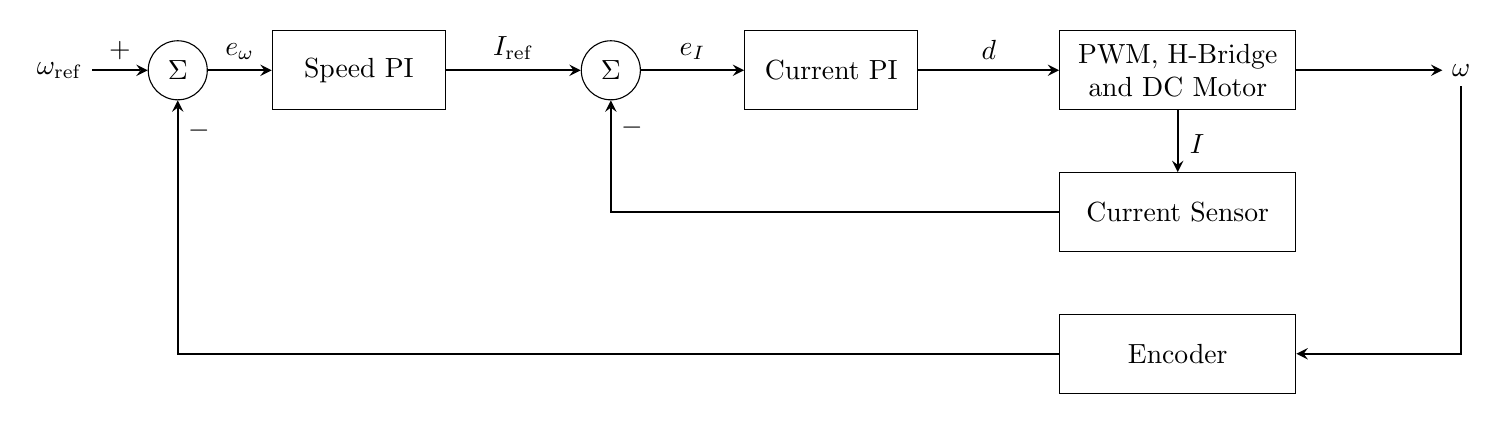
\begin{tikzpicture}[
        >=stealth,
        block/.style={draw, rectangle, minimum width=2.2cm,
                      minimum height=1.0cm, align=center},
        sum/.style={draw, circle, minimum size=0.75cm, inner sep=0pt},
        signal/.style={->, thick}
    ]
        \node (wref) at (0,0) {$\omega_{\mathrm{ref}}$};
        \node[sum] (sumw) at (1.5,0) {$\Sigma$};
        \node[block] (speedpid) at (3.8,0) {Speed PI};
        \node[sum] (sumi) at (7.0,0) {$\Sigma$};
        \node[block] (currentpid) at (9.8,0) {Current PI};
        \node[block, minimum width=3.0cm] (plant) at (14.2,0)
            {PWM, H-Bridge\\and DC Motor};
        \node (wout) at (17.8,0) {$\omega$};

        \node[block, minimum width=3.0cm] (currentfb) at (14.2,-1.8)
            {Current Sensor};
        \node[block, minimum width=3.0cm] (encoder) at (14.2,-3.6)
            {Encoder};

        \draw[signal] (wref) -- node[above] {$+$} (sumw);
        \draw[signal] (sumw) -- node[above] {$e_{\omega}$} (speedpid);
        \draw[signal] (speedpid) -- node[above] {$I_{\mathrm{ref}}$} (sumi);
        \draw[signal] (sumi) -- node[above] {$e_I$} (currentpid);
        \draw[signal] (currentpid) -- node[above] {$d$} (plant);
        \draw[signal] (plant) -- (wout);

        \draw[signal] (plant.south) -- node[pos=0.55, right=3pt, fill=white,
                                             inner sep=1pt] {$I$}
                                      (currentfb.north);
        \draw[signal] (currentfb.west) -| node[pos=0.88, right] {$-$} (sumi.south);

        \draw[signal] (wout.south) |- (encoder.east);
        \draw[signal] (encoder.west) -| node[pos=0.94, right] {$-$} (sumw.south);
    \end{tikzpicture}%
    }
    \caption{串级 PI 控制结构框图。}
    \label{fig:cascade}
\end{figure}

\begin{table}[H]
    \centering
    \caption{串级 PI 框图中的符号说明。}
    \label{tab:cascade_symbols}
    \begin{tabular}{lll}
        \toprule
        \textbf{符号} & \textbf{含义} & \textbf{单位或范围} \\
        \midrule
        $\omega_{\mathrm{ref}}$ & 目标转速 & RPM \\
        $\omega$                & 实际转速 & RPM \\
        $e_{\omega}$            & 转速误差，$\omega_{\mathrm{ref}}-\omega$ & RPM \\
        $I_{\mathrm{ref}}$      & 速度外环输出的目标电流 & 0--400\,mA \\
        $I$                     & 电流检测模块测得的实际电流 & mA \\
        $e_I$                   & 电流误差，$I_{\mathrm{ref}}-I$ & mA \\
        $d$                     & 发送给 FPGA 的 PWM 占空比数值 & 0--4095 \\
        \bottomrule
    \end{tabular}
\end{table}

串级控制通常要求内环的动态响应快于外环~\cite{astrom2006}。本项目的速度环和电流环均以 1\,kHz 频率计算，但两者作用不同：速度环根据转速误差生成目标电流，电流环则根据目标电流与实测电流之间的误差直接调整 PWM 指令。由于电流变化通常快于机械转速变化，电流环可以在转速发生明显变化之前对电流偏差进行调节。

\section{速度外环设计}

本项目根据电机运行情况逐步调整 PI 参数。调试时先调整比例增益 $K_p$，观察系统是否出现明显振荡；再调整决定误差累积作用大小的积分增益 $K_i$，减小系统稳定后目标值与实际值之间的差值，同时避免实际值在响应过程中明显超过目标值。

速度外环根据目标转速与实际转速的误差计算目标电流，当前参数见表~\ref{tab:speed_pid}。

\begin{table}[H]
    \centering
    \caption{速度外环 PI 参数。}
    \label{tab:speed_pid}
    \begin{tabular}{lll}
        \toprule
        \textbf{参数} & \textbf{数值} & \textbf{说明} \\
        \midrule
        $K_p$ & 1.5 & 100\,RPM 误差时比例项为 150\,mA \\
        $K_i$ & 0.1 & 用于减小稳态转速误差 \\
        $u_{\min}$ & 0\,mA & 目标电流下限 \\
        $u_{\max}$ & 400\,mA & 目标电流上限 \\
        $I_{\max}$ & 4000 & 积分项最大贡献为 400\,mA \\
        \bottomrule
    \end{tabular}
\end{table}

\section{电流内环设计}

电流内环根据目标电流与实测电流的误差计算 12 位 PWM 指令。调试中，$K_p=20$、$K_i=0.5$ 时占空比振荡明显，降低增益后得到表~\ref{tab:current_pid}所示参数。

\begin{table}[H]
    \centering
    \caption{电流内环 PI 参数。}
    \label{tab:current_pid}
    \begin{tabular}{lll}
        \toprule
        \textbf{参数} & \textbf{数值} & \textbf{说明} \\
        \midrule
        $K_p$ & 5.0 & 调整后占空比振荡减小 \\
        $K_i$ & 0.2 & 用于减小稳态电流误差 \\
        $u_{\min}$ & 0 & PWM duty下限 \\
        $u_{\max}$ & 4095 & 12 位 PWM duty上限 \\
        $I_{\max}$ & 8000 & 积分项最大贡献为 1600 \\
        \bottomrule
    \end{tabular}
\end{table}

两个环路的增益数值不能直接比较。速度环 $K_p$ 的单位为 $\mathrm{mA/RPM}$，电流环 $K_p$ 的单位为 PWM 计数每毫安（count/mA）；两者的输入、输出及量程均不同。

以上参数用于当前空载调试。

\section{1\,kHz 控制循环实现}

TIM6 每 1\,ms 产生一次更新中断。编码器读取、ADC 转换、两级 PI 运算和 SPI 发送均在该中断中完成，因此这些操作的总执行时间必须小于 1\,ms。

\texttt{TIM6\_DAC\_IRQHandler} 每 1\,ms 执行一次，执行顺序如下：

\begin{enumerate}
    \item 更新编码器：计算 $\Delta_{\text{count}}$ 并更新滤波后 RPM。
    \item 读取电位器 ADC（16 点均值滤波），并进行零位处理。
    \item \textbf{速度 PI}：$e_\omega = \omega_{\text{ref}} - \omega_{\text{meas}}
          \;\Rightarrow\; I_{\text{ref}}\in[0,400]\,\text{mA}$。
    \item 读取电流 ADC（8 点均值滤波）。
    \item \textbf{电流 PI}：$e_I = I_{\text{ref}} - I_{\text{meas}}
          \;\Rightarrow\; d \in [0, 4095]$。
    \item 通过 SPI2 向 FPGA 发送占空比 $d$（2 字节）。
\end{enumerate}

ADC 时钟为 21\,MHz。电位器和电流通道的采样时间分别为 144 和 28 个 ADC 时钟周期，12 位转换还需要 12 个周期，因此两路转换时间为
\[
    t_{\mathrm{ADC}}
    =\frac{144+12}{21\,\mathrm{MHz}}
     +\frac{28+12}{21\,\mathrm{MHz}}
    \approx 9.33\,\mu\mathrm{s}.
\]
SPI2 时钟为 5.25\,MHz，发送两个字节共需 16 个 SCK 周期：
\[
    t_{\mathrm{SPI}}=\frac{16}{5.25\,\mathrm{MHz}}
    \approx 3.05\,\mu\mathrm{s}.
\]
两者合计约 12.38\,$\mu$s。经测试1ms的中断周期足够使用。

% ════════════════════════════════════════════════════════════════════════════
%  第五章 — FPGA 开发
% ════════════════════════════════════════════════════════════════════════════
\chapter{FPGA 开发}

FPGA 设计包含三个 VHDL 模块，使用 Xilinx ISE 14.7 综合，目标器件为 Spartan-6 XC6SLX9-2FTG256。

\section{SPI 从机接收器（\texttt{spi\_slave.vhd}）}

\subsection{跨时钟域同步}

传统 SPI 从机可以直接使用 SCK 驱动移位寄存器，再将完整数据传入 FPGA 系统时钟域。本项目的 SCK 为 5.25\,MHz，低于 FPGA 的 50\,MHz 系统时钟，因此采用系统时钟过采样 SCK 的实现方式，使 SPI 接收和后续 PWM 逻辑都工作在 50\,MHz 时钟域；类似实现可见 FPGA4Fun 的 SPI 从机示例~\cite{fpga4fun_spi}。

SCK 来自 STM32，与 FPGA 内部时钟没有固定相位关系。若直接采样，采样时刻落在 SCK 跳变沿附近时可能产生亚稳态。程序使用两个串联触发器对 SCK 进行同步，并根据两级采样值检测上升沿。第一级接收异步输入，第二级在下一时钟周期再次采样，从而降低亚稳态传播到后级逻辑的概率。核心代码如下：

\begin{lstlisting}[style=vhdlstyle, caption={SCK 两级同步链。}]
p_sync : process(clk)
begin
    if rising_edge(clk) then
        sck_d1 <= sck;
        sck_d2 <= sck_d1;
    end if;
end process;
sck_rise <= sck_d1 and (not sck_d2);  -- 单周期上升沿脉冲
\end{lstlisting}

\subsection{两字节帧接收与占空比重组}

PWM 占空比为 12 位，而 SPI2 采用 8 位数据帧，因此 STM32 将占空比拆成两个字节发送。第一个字节的低 4 位存放 $d[11:8]$，第二个字节存放 $d[7:0]$，其重组关系为
\[
    d[11:0]=\{\text{Byte0}[3:0],\,\text{Byte1}[7:0]\}.
\]

CS\_N 拉低后，FPGA 在每个 SCK 上升沿采样一位 MOSI 数据，并通过 \texttt{bit\_cnt} 记录已接收的位数。前 8 位接收完成后，程序保存第一个字节的低 4 位；后 8 位接收完成后，将两部分拼接为 12 位 \texttt{duty\_out}。CS\_N 上升表示一帧传输结束，模块产生一个时钟周期的 \texttt{duty\_valid} 信号，使 PWM 模块更新占空比。核心代码如下：

\begin{lstlisting}[style=vhdlstyle, caption={SPI 数据移位与占空比拼接。}]
if cs_rise = '1' then
    duty_valid <= '1';
    bit_cnt    <= 0;
    shift_reg  <= (others => '0');

elsif sck_rise = '1' and cs_d1 = '0' then
    shift_reg <= shift_reg(6 downto 0) & mosi_d1;

    if bit_cnt = 7 then
        temp_hi <= shift_reg(2 downto 0) & mosi_d1;
        bit_cnt <= 8;
    elsif bit_cnt = 15 then
        duty_out <= temp_hi & (shift_reg(6 downto 0) & mosi_d1);
        bit_cnt  <= 0;
    else
        bit_cnt <= bit_cnt + 1;
    end if;
end if;
\end{lstlisting}

\section{PWM 发生器（\texttt{pwm\_gen.vhd}）}

12 位自由计数器与锁存的占空比寄存器进行比较：

\begin{lstlisting}[style=vhdlstyle, caption={PWM 比较器。}]
pwm_out <= '1' when (pwm_cnt < duty_reg) else '0';
\end{lstlisting}

SPI 从机产生的 \texttt{duty\_valid} 选通信号仅在帧边界处更新 \texttt{duty\_reg}，防止在 PWM 周期中途产生毛刺。

\section{顶层集成（\texttt{top.vhd}）}

\texttt{top.vhd} 将 SPI 接收模块与 PWM 模块连接起来。SPI 接收模块输出 12 位占空比及数据有效信号，PWM 模块收到有效信号后更新占空比并产生 PWM 输出。各输入输出信号对应的 FPGA 引脚由 \texttt{pin.ucf} 指定，具体分配见表~\ref{tab:fpga_pins}。

\begin{table}[H]
    \centering
    \caption{FPGA 引脚分配（AX309 J3 扩展接口）。}
    \label{tab:fpga_pins}
    \begin{tabular}{llll}
        \toprule
        \textbf{信号} & \textbf{FPGA 引脚} & \textbf{J3 针脚} & \textbf{连接对象} \\
        \midrule
        clk      & P8  & 板载晶振 & --- \\
        sck      & C15 & J3-21 & STM32 PB13 \\
        cs\_n    & D16 & J3-23 & STM32 PB12 \\
        mosi     & C16 & J3-24 & STM32 PB15 \\
        miso     & E15 & J3-26 & STM32 PB14（不使用） \\
        pwm\_out & F16 & J3-31 & TB6612 PWMA \\
        \bottomrule
    \end{tabular}
\end{table}

% ════════════════════════════════════════════════════════════════════════════
%  第六章 — 系统集成与测试
% ════════════════════════════════════════════════════════════════════════════
\chapter{系统集成与测试}

本章介绍系统集成后的测试结果和调试中发现的问题。目前已完成 FPGA PWM 频率、Flash 参数保存和电流采样测试；转速稳态误差、阶跃响应和带负载电流响应仍需补测。

\section{测试内容与方法}

完成 STM32F407、AX309 FPGA、电机驱动模块、INA240A2 和编码器的连接后，对系统进行测试。测试结果分为三类：实物照片记录硬件连接和 OLED 显示；串口与逻辑分析仪截图记录参数存储、SPI 和 PWM 信号；串口运行数据用于绘制转速、电流和 PWM 曲线。具体方法见表~\ref{tab:test_methods}。

\begin{table}[H]
    \centering
    \caption{系统功能测试项目。}
    \label{tab:test_methods}
    \begin{tabular}{p{3.2cm}p{4.2cm}p{5.1cm}}
        \toprule
        \textbf{测试项目} & \textbf{工具或条件} & \textbf{测试方法} \\
        \midrule
        系统运行状态 & 相机，OLED 显示 &
            拍摄硬件连接及 OLED 显示的转速、电流和 PWM 数据 \\
        FPGA PWM 输出 & 逻辑分析仪，J3-31 引脚 &
            测量 PWM 周期并与理论频率比较 \\
        Flash 参数保存 & 串口命令，W25Q64 &
            保存 PI 参数，断电后重新上电并读取 \\
        电流采样 & 100\,RPM，输出轴无外接负载 &
            记录 ADC 换算后的电机电流 \\
        闭环运行过程 & UART 连续输出运行数据 &
            按时间绘制转速、电流和 PWM 曲线 \\
        \bottomrule
    \end{tabular}
\end{table}

为便于后续处理，串口以固定周期输出以下字段：
\begin{verbatim}
time_ms,target_rpm,measured_rpm,current_ref_mA,current_mA,pwm
\end{verbatim}
串口输出频率应低于控制循环频率，例如每 10--20\,ms 输出一次，避免串口发送影响 1\,kHz 控制中断。

\section{实验结果}

\subsection{系统运行状态}

系统上电后，OLED 显示目标转速、实际转速、PWM 占空比和电机电流。实物照片可以说明系统已经正常运行，但转速响应仍需通过连续数据曲线分析。

\begin{figure}[H]
    \centering
    \IfFileExists{images/system_oled.jpg}{
        \includegraphics[width=0.8\textwidth]{images/system_oled.jpg}
    }{
        \fbox{\parbox{0.75\textwidth}{\centering\vspace{2cm}
        待插入：系统硬件连接与 OLED 运行状态照片
        \vspace{2cm}}}
    }
    \caption{系统实物及 OLED 运行状态。}
    \label{fig:system_oled}
\end{figure}

\subsection{FPGA PWM 输出}

FPGA 使用 50\,MHz 时钟驱动 12 位计数器，PWM 理论频率为
\[
    f_{\mathrm{PWM}}=\frac{50\,\mathrm{MHz}}{4096}
    =12.20703125\,\mathrm{kHz}.
\]
逻辑分析仪测得 J3-31 引脚的 PWM 频率为 12.207\,kHz，与理论计算结果一致，说明 FPGA 计数器和 PWM 输出工作正常。

\begin{figure}[H]
    \centering
    \IfFileExists{images/pwm_waveform.png}{
        \includegraphics[width=0.85\textwidth]{images/pwm_waveform.png}
    }{
        \fbox{\parbox{0.8\textwidth}{\centering\vspace{1.5cm}
        待插入：逻辑分析仪测得的 PWM 波形与频率截图
        \vspace{1.5cm}}}
    }
    \caption{FPGA PWM 输出波形。}
    \label{fig:pwm_waveform}
\end{figure}

\subsection{W25Q64 参数存储}

W25Q64 读取到的器件标识为 \texttt{0xEF16}。通过串口修改并保存 PI 参数后，断电再上电仍能读到保存值，说明参数保存和上电加载功能正常。

\begin{figure}[H]
    \centering
    \IfFileExists{images/flash_power_cycle.png}{
        \includegraphics[width=0.85\textwidth]{images/flash_power_cycle.png}
    }{
        \fbox{\parbox{0.8\textwidth}{\centering\vspace{1.5cm}
        待插入：参数保存及断电重启后自动加载的串口截图
        \vspace{1.5cm}}}
    }
    \caption{W25Q64 参数保存与上电加载结果。}
    \label{fig:flash_power_cycle}
\end{figure}

\subsection{ADC 电流采样}

零电流时 ADC 原始值约为 2200，对应 INA240A2 输出约 1.773\,V，程序将该值作为零点。在输出轴未连接外部负载、目标转速为 100\,RPM 时，测得电机电流约为 30\,mA。该结果说明 ADC 能够读出电机运行时的电流变化。由于尚未使用独立电流表进行对比，本节不评价测量精度。

\begin{figure}[H]
    \centering
    \IfFileExists{images/current_measurement.png}{
        \includegraphics[width=0.85\textwidth]{images/current_measurement.png}
    }{
        \fbox{\parbox{0.8\textwidth}{\centering\vspace{1.5cm}
        待插入：零电流 ADC 值及 100\,RPM 空载电流的串口截图
        \vspace{1.5cm}}}
    }
    \caption{ADC 电流采样结果。}
    \label{fig:current_measurement}
\end{figure}

\subsection{闭环转速控制}

系统能够读取编码器转速，并根据 PI 计算结果更新 PWM 指令。测试时通过 UART 连续记录目标转速、实际转速、目标电流、实测电流和 PWM 指令，再按时间绘制曲线。转速曲线用于计算稳态误差、上升时间和超调量；电流和 PWM 曲线用于观察启动和调速过程。

\begin{figure}[H]
    \centering
    \IfFileExists{images/speed_response.png}{
        \includegraphics[width=0.85\textwidth]{images/speed_response.png}
    }{
        \fbox{\parbox{0.8\textwidth}{\centering\vspace{1.5cm}
        待测试并插入：0--100\,RPM 闭环阶跃响应曲线
        \vspace{1.5cm}}}
    }
    \caption{闭环转速阶跃响应。}
    \label{fig:speed_response}
\end{figure}

\begin{figure}[H]
    \centering
    \IfFileExists{images/current_pwm_response.png}{
        \includegraphics[width=0.85\textwidth]{images/current_pwm_response.png}
    }{
        \fbox{\parbox{0.8\textwidth}{\centering\vspace{1.5cm}
        待测试并插入：目标电流、实测电流及 PWM 随时间变化曲线
        \vspace{1.5cm}}}
    }
    \caption{电流与 PWM 动态响应。}
    \label{fig:current_pwm_response}
\end{figure}

\section{调试问题与处理}

表~\ref{tab:issues} 列出了系统调试中遇到的主要问题和处理方法。

\begin{table}[H]
    \centering
    \caption{主要调试问题及处理方法。}
    \label{tab:issues}
    \begin{tabular}{p{2.8cm}p{4cm}p{5.7cm}}
        \toprule
        \textbf{问题} & \textbf{现象} & \textbf{原因与处理方法} \\
        \midrule
        串口无输出 &
            ST-Link 虚拟串口无数据 &
            改用外接 CH340G，并通过 PA2、PA3 连接 USART2。 \\
        \addlinespace
        电流换算错误 &
            电流读数偏高约 2.5 倍 &
            INA240 为 A2 版，增益应为 50\,V/V；修正软件中的增益参数。 \\
        \addlinespace
        电流环振荡 &
            PWM 占空比大幅波动 &
            降低电流环参数，将 $K_p$ 从 20 调整为 5，$K_i$ 从 0.5 调整为 0.2。 \\
        \addlinespace
        编码器无反馈 &
            RPM 为 0，PWM 持续增大 &
            编码器供电未连接；恢复供电后转速反馈恢复正常。 \\
        \addlinespace
        电位器零点偏置 &
            零位仍产生较小转速给定 &
            零位 ADC 读数约为 9，程序将小于 50 的读数处理为 0。 \\
        \addlinespace
        Flash 写入失败 &
            保存后断电丢失，回读为 \texttt{0xFFFFFFFF} &
            CS 两次操作之间的间隔不足；增加 CS 拉高后的等待时间，并加入写后回读验证。 \\
        \bottomrule
    \end{tabular}
\end{table}

\section{本章小结}

现有测试表明，FPGA PWM 输出、W25Q64 参数保存和 INA240A2 电流采样功能正常。系统已经能够闭环运行，但还缺少不同目标转速下的稳态误差、0--100\,RPM 阶跃响应和带负载电流数据。完成这些测试后，才能分析串级 PI 的控制效果。

% ════════════════════════════════════════════════════════════════════════════
%  参考文献
% ════════════════════════════════════════════════════════════════════════════
\bibliographystyle{IEEEtran}
\begin{thebibliography}{9}

\bibitem{rm0090}
STMicroelectronics,
\textit{RM0090: STM32F405/407/415/417 Reference Manual},
Rev.\ 19, 2021. [Online]. Available: \url{https://www.st.com}

\bibitem{ds8626}
STMicroelectronics,
\textit{DS8626: STM32F407VG Datasheet},
Rev.\ 9, 2021.

\bibitem{ina240}
Texas Instruments,
\textit{INA240 Bidirectional, Low- and High-Side, Voltage Output,
Current-Sense Amplifier Datasheet}, SBOS566D, 2015.

\bibitem{w25q64}
Winbond Electronics,
\textit{W25Q64FV 64M-bit Serial Flash Memory Datasheet},
Rev.\ L, 2017.

\bibitem{tb6612}
Toshiba,
\textit{TB6612FNG Dual DC Motor Driver IC Datasheet},
2015.

\bibitem{ssd1306}
Solomon Systech,
\textit{SSD1306 Dot Matrix OLED/PLED Segment/Common Driver with
Controller Datasheet}, 2008.

\bibitem{astrom2006}
K.~J. \AA{}str\"{o}m and T.~H\"{a}gglund,
\textit{Advanced PID Control}.
ISA -- The Instrumentation, Systems, and Automation Society, 2006.

\bibitem{fpga4fun_spi}
FPGA4Fun,
``SPI 2---A Simple Implementation,'' [Online].
Available: \url{https://www.fpga4fun.com/SPI2.html}.

\end{thebibliography}

% ════════════════════════════════════════════════════════════════════════════
%  附录
% ════════════════════════════════════════════════════════════════════════════
\appendix

\chapter{关键源代码}

\section{TIM6 1\,kHz PI 控制循环}

\begin{lstlisting}[style=cstyle, caption={TIM6\_DAC\_IRQHandler：1\,kHz 串级 PI 控制循环。}]
void TIM6_DAC_IRQHandler(void)
{
    if (TIM6->SR & TIM_SR_UIF) {
        TIM6->SR &= ~TIM_SR_UIF;

        Encoder_Update();

        uint16_t adc_val      = ADC1_Read_Filtered();
        float    setpoint_rpm = (adc_val < 50U) ? 0.0f
                             : (float)adc_val * (MOTOR_MAX_RPM / 4095.0f);

        float current_setpoint = PID_Calc(&speed_pid,
                                          setpoint_rpm, g_encoder_rpm);

        float measured_current = ADC1_ReadCurrent_Filtered_mA();

        float    duty_f = PID_Calc(&current_pid,
                                   current_setpoint, measured_current);
        uint16_t duty   = (uint16_t)duty_f;

        uint8_t hi = (duty >> 8U) & 0x0FU;
        uint8_t lo =  duty        & 0xFFU;
        FPGA_CS_LOW();
        SPI2_ReadWriteByte(hi);
        SPI2_ReadWriteByte(lo);
        FPGA_CS_HIGH();

        g_pid_duty = duty;
    }
}
\end{lstlisting}

\section{位置式 PID 实现}

\begin{lstlisting}[style=cstyle, caption={PID\_Calc：带抗积分饱和的位置式PID。}]
float PID_Calc(PID_TypeDef *pid, float setpoint, float feedback)
{
    float err = setpoint - feedback;

    pid->integral += err;
    if      (pid->integral >  pid->integral_max)
        pid->integral =  pid->integral_max;
    else if (pid->integral < -pid->integral_max)
        pid->integral = -pid->integral_max;

    float deriv = pid->kd * (err - pid->err_prev);
    pid->err_prev = err;

    float output = pid->kp * err + pid->ki * pid->integral + deriv;

    if (output > pid->out_max) {
        output = pid->out_max;
        if (err > 0.0f) pid->integral -= err;
    } else if (output < pid->out_min) {
        output = pid->out_min;
        if (err < 0.0f) pid->integral -= err;
    }
    return output;
}
\end{lstlisting}

\end{document}
